%!TEX root = ../../PhD_thesis__Edouard_Leurent

\graphicspath{{2-Chapters/1-Chapter/}}

\chapter{Introduction}
\label{chapter:1}

\begin{flushright}
	\begin{tabular}{@{}l@{}}
		\emph{Pour soulever un poids si lourd,}\\
		\emph{Sisyphe, il faudrait ton courage !}\\
		\emph{Bien qu’on ait du cœur à l’ouvrage,}\\
		\emph{L’Art est long et le Temps est court.}\\
	\end{tabular}

	Charles Baudelaire, \href{https://eleurent.github.io/sisyphe/texts/le-guignon.html}{\emph{Le guignon}}.
\end{flushright}

\section{Context and scope}


\paragraph{How should a self-driving car act?}

In the first few weeks of my PhD, I made the following observation: when confronted to this question, say at the occasion of a social dinner, layman interlocutors have a general tendency to conjure up disaster scenarios involving imminent accidents with unavoidable casualties. 
This reflex is likely to stem from the popularisation of the Trolley Problem \citep{Foot1967}, a famous thought experiment in Moral Philosophy, depicted in \Cref{fig:trolley}, in which a runaway trolley is headed straight toward five people tied up on the main track and unable to move. A lever, when pulled, switches the trolley to a side track occupied by one person. What should you do? The field of normative ethics focuses on answering the question of what we \emph{ought} to do, and this dilemma illustrates a clash between two schools of thought: utilitarianism and deontological ethics. 
It has been transposed in the context of Autonomous Driving, for instance in the \emph{Moral Machine} platform \citep{Awad2018}.

\begin{figure}[tp]
	\centering
	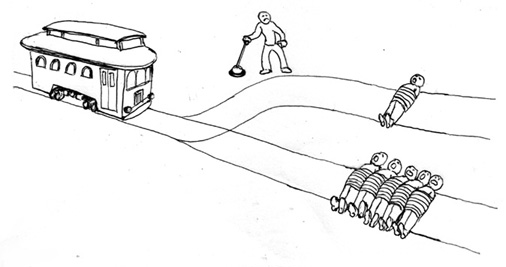
\includegraphics[width=0.7\linewidth]{img/trolley}
	\caption{The Trolley Problem \citep{Foot1967}. Image by \href{http://subcortex.com/}{Jesse J. Prinz}.}
	\label{fig:trolley}
\end{figure}

% Ethics is a branch of philosophy studying what is the right (or wrong) action to take in any situation. 
Yet when we drive, we seldom find ourselves in such extreme situations, and our thoughts typically focus on less tragic questions than who to sacrifice.
Likewise, this thesis is not so much about solving moral dilemma than addressing the non-dilemma of how to avoid accidents altogether.%, which ultimately implies also avoiding such states of unavoidable collision.

\paragraph{Architecture of self-driving software}

The robotics pipeline typically involves three modules: Perception, Decision, and Control.
Great research efforts have been made to resolve the two end-of-pipe tasks: Perception has benefited from the substantial progress in the field of Computer Vision due to the recent advent of Deep Learning, and Control schemes have been developed for ground vehicles to precisely follow a predefined trajectory. Nowadays, ADAS systems support features such as LKA, ACC. However, we claim that Decision has been a neglected area: hitherto, most applications and challenges focused on simple highway settings with little 

% What problems do we have to face?
% Decision making in the presence of uncertainty.
% Perception is hard, known to be long tail.
% Assume we have magically access to magical perception. Would we have solved the problem?
% We still need to decide of how to act. Even if the present were known, the future would still be uncertain, because we do not know how other agents are going to act.
% Human driving behaviour is not deterministic, but it is predictable. Highly structured.
% Recall aletoric vs epistemic uncertainty?

% Our objectives: 
% 1. Socially aware decision-making (account for other agents, and how our actions impact their behaviours)
% 2. A notion of safety. Risk as a constraint ? As a worst-case outcome?




\section{Our contributions}
\section{Outline}

% Is this needed? Merge with contributions?

\section{List of publications}